\documentclass{report}
\usepackage{ctex}
\usepackage{graphicx}
\usepackage{amsmath}
\usepackage{indentfirst}
\usepackage{titlesec}
\usepackage{setspace}
\usepackage{subfigure}
\usepackage{caption}
\usepackage{float}
\usepackage{booktabs}
\usepackage{geometry}
\usepackage{multirow}
\geometry{left=1cm,right=1cm,top=3cm}
\title{\songti \zihao{2}\bfseries 液晶光电效应综合实验}
\titleformat*{\section}{\songti\zihao{4}\bfseries}
\titleformat*{\subsection}{\songti\zihao{5}\bfseries}
\renewcommand\thesection{\arabic{section}}
\author{王启骅 PB20020580}
\begin{document}
	\maketitle
	\section{实验目的}
	掌握液晶光开关的基本工作原理的基础上,测量液晶光开关的电光特性曲线,并由电光特性曲线得到液晶的阈值电压和关断电压。测量液晶光开关的时间响应曲线,得到液晶的上升时间和下降时间。测量由液晶光开关矩阵所构成的液晶显示器的视角特性以及在不同视角下的对比度。了解液晶光开关构成图像矩阵的方法。
	\section{实验原理}
	无电场时,液晶层均匀扭曲排列起来的结构具有光波导的性质,扭曲排列起来的液晶传播到下电极表面时,偏振方向会旋转 90 度,来自光源的自然光经过偏振片 P1 变为平行于透光轴的线偏振光,到达输出面时,偏振面旋转 90度,与 P2 的透光轴平
	行,光通过。在施加足够电压,静电场的作用下,液晶分子趋于平行于电场方向排列,成均匀结构,从 P1 透射出来的偏振光的偏振方向在液晶中传播时不再旋转,光被关断。
	
	
	当光线垂直液晶面入射时,透射率随外加电压的升高而逐渐降低,在一定电压下达到最
	低点。可以根据测得电光特性曲线图得出液晶的阈值电压和关断电压。
	
	
	加上(或去掉)驱动电压能使液晶的开关状态发生改变,是因为液晶的分子排序发生了改变需要一定时间,上升时间 $ \tau_r $和下降时间$ \tau_d $。给液晶开关加上周期性变化的电压,就可以得到液晶的时间响应曲线,上升时间和下降时间。
	
	
	液晶光开关的视角特性表示对比度与视角的关系。对比度大于 5 时图像清晰,对比度小于 2,图像就模糊不清。对比度与垂直视角、水平视角有关,具有非对称性。
	
	
	矩阵型显示器的工作方式为扫描方式。通过逐行、列加不同高低电平的方式显示像素。
	\section{实验仪器}
	液晶光开关电光特性综合实验仪、示波器、计算机。
	\section{数据处理}
	\subsection{液晶光开关电光特性测量}
	\begin{table}[!h]
		\centering
		\captionsetup{font={small},labelfont=bf}
		\caption{\heiti\zihao{-5}液晶光开关电光特性测量}
		\begin{tabular}{|c|c|c|c|c|c|c|c|c|c|c|c|c|c|c|c|c|c|}
			
			\hline
			\multicolumn{2}{|c|}{电压(V)}&0&0.5&0.8&1.0&1.1&1.2&1.3&1.4&1.5&1.6&1.7&2.0&3.0&4.0&5.0&6.0\\
			\hline
			\multirow{4}{*}{透射率$ /\% $}&1&100&99.7&86.0&51.9&35.7&23.1&14.6&9.3&6.3&4.8&4.2&4.3&4.7&4.2&3.8&3.5\\
			\cline{2-18}
			\multirow{4}{*}{}&2&99.9&99.6&85.7&52.2&35.8&23.2&14.3&9.2&6.2&4.8&4.2&4.3&4.7&4.2&3.8&3.5\\
			\cline{2-18}
			\multirow{4}{*}{}&3&100&99.8&85.9&51.9&35.7&22.9&14.4&9.2&6.3&4.8&4.2&4.3&4.7&4.2&3.8&3.5\\
			\cline{2-18}
			\multirow{4}{*}{}&平均&100&99.7&85.9&52.0&35.7&23.1&14.4&9.2&6.3&4.8&4.2&4.3&4.7&4.2&3.8&3.5\\
			\hline
			
			
			
			
			
			
		\end{tabular}
	\end{table}
	依据实验数据绘制电光特性曲线:
	\begin{figure}
		\centering
		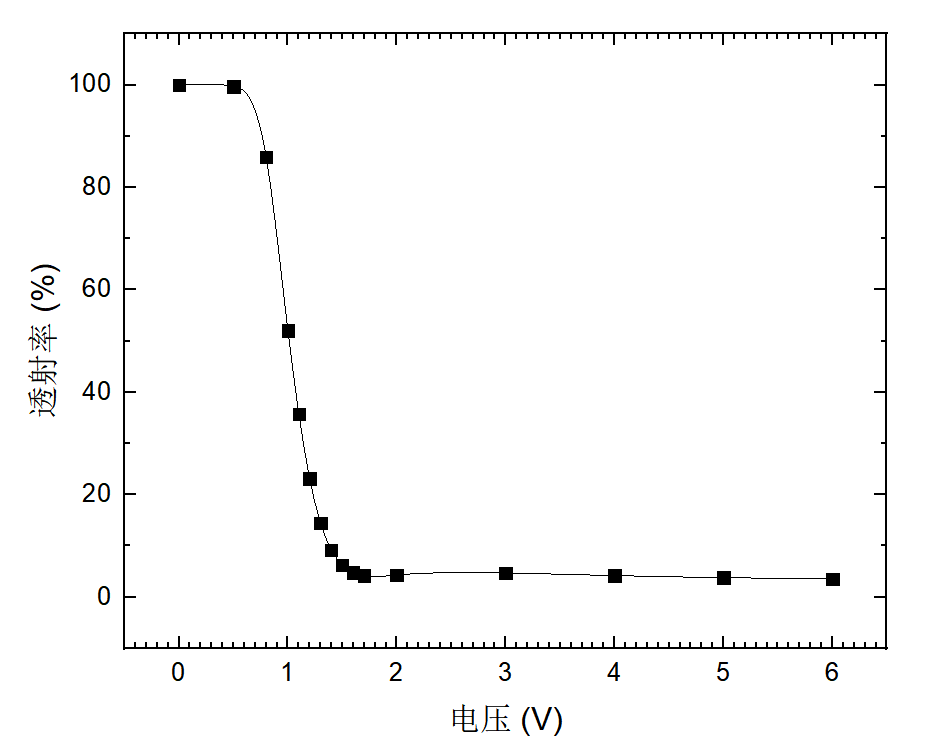
\includegraphics[scale=0.5]{电压}
		\captionsetup{font={small},labelfont=bf}
		\caption{\heiti\zihao{-5}电光特性曲线}
		
	\end{figure}
	
	
	根据该曲线图得到阈值电压=0.73V,关断电压=1.39V
	\subsection{液晶的时间响应的测量}
	\begin{table}[!h]
		\centering
		\captionsetup{font={small},labelfont=bf}
		\caption{\heiti\zihao{-5}响应时间}
		\begin{tabular}{|c|c|c|c|c|}
			
			\hline
			次数&1&2&3&平均\\
			\hline
			$ \tau_r/ms $&45.00&44.00&45.20&44.73\\
			\hline
			$ \tau_d/ms $&23.00&22.40&22.00&22.47\\
			\hline
			
		\end{tabular}
	\end{table}
	计算得到
	\begin{equation}
		\tau_r=44.73ms \nonumber
	\end{equation}
	\begin{equation}
		\tau_d=22.47ms \nonumber
	\end{equation}
	\subsection{液晶光开关视角特性的测量}
	\begin{table}[!h]
		\centering
		\captionsetup{font={small},labelfont=bf}
		\caption{\heiti\zihao{-5}水平方向视角特性}
		\begin{tabular}{|c|c|c|c|c|c|c|c|c|c|c|c|c|c|c|c|c|}
			
			\hline
			正角度&0&5&10&15&20&25&30&35&40&45&50&55&60&65&70&75\\
			\hline
			$ T_{max} $&100&100&100&100&100&99.6&97.6&95.5&94.6&90.0&86.8&79.6&72.1&61.8&49.7&32.9\\
			\hline
			$ T_{min} $&4.3&4.2&4.1&3.9&3.7&3.7&3.7&3.6&3.5&3.5&3.6&3.7&3.8&3.8&3.4&2.8\\
			\hline
			$ T_{max}/T_{min} $&23.3&23.8&24.4&25.6&27.0&26.9&26.4&26.5&27.0&25.7&24.1&21.5&19.0&16.3&14.6&11.8\\
			\hline
			负角度&0&5&10&15&20&25&30&35&40&45&50&55&60&65&70&75\\
			\hline
			$ T_{max} $&100&99.9&99.9&99.9&99.6&98.8&96.5&94.1&92.8&87.9&84.2&77.5&69.9&60.7&48.7&35.5\\
			\hline
			$ T_{min} $&4.3&4.3&4.2&4.0&3.8&3.7&3.6&3.5&3.5&3.5&3.7&3.7&3.8&3.8&3.4&2.8\\
			\hline
			$ T_{max}/T_{min}$&23.3&23.2&23.8&25.0&26.2&26.7&26.8&26.9&26.5&25.1&22.8&20.9&18.4&16.0&14.3&12.7\\
			\hline
			
			
			
		\end{tabular}
	\end{table}
	\begin{table}[!h]
		\centering
		\captionsetup{font={small},labelfont=bf}
		\caption{\heiti\zihao{-5}垂直方向视角特性}
		\begin{tabular}{|c|c|c|c|c|c|c|c|c|c|c|c|c|c|c|c|c|}
			
			\hline
			正角度&0&5&10&15&20&25&30&35&40&45&50&55&60&65&70&75\\
			\hline
			$ T_{max} $&100&99.4&98.4&96.6&94.2&91.4&89.1&85.9&82.8&80.7&78.6&76.3&73.1&66.7&55.9&40.8\\
			\hline
			$ T_{min} $&4.2&5.9&9.1&14.2&20.3&27.6&35.5&43.6&50.9&57.9&63.4&66.3&67.1&63.3&54.5&41.0\\
			\hline
			$ T_{max}/T_{min} $&23.8&16.8&10.8&6.80&4.64&3.31&2.51&2.02&1.62&1.39&1.24&1.15&1.09&1.05&1.03&0.995\\
			\hline
			负角度&0&5&10&15&20&25&30&35&40&45&50&55&60&65&70&75\\
			\hline
			$ T_{max} $&100&100&99.4&98.2&96.2&93.8&91.6&88.4&84.9&81.7&77.6&72.8&67.4&60.0&50.6&38.0\\
			\hline
			$ T_{min} $&4.2&4.0&5.2&7.8&12.0&17.9&25.5&34.3&44.1&53.6&61.1&65.1&65.3&61.2&52.9&40.3\\
			\hline
			$ T_{max}/T_{min}$&23.8&25.0&19.1&12.6&8.01&5.24&3.59&2.57&1.93&1.52&1.27&1.12&1.03&0.980&0.957&0.943\\
			\hline
			
			
			
		\end{tabular}
	\end{table}
	\begin{figure}[!h]
		
		\centering
		\subfigure[水平方向负角度]{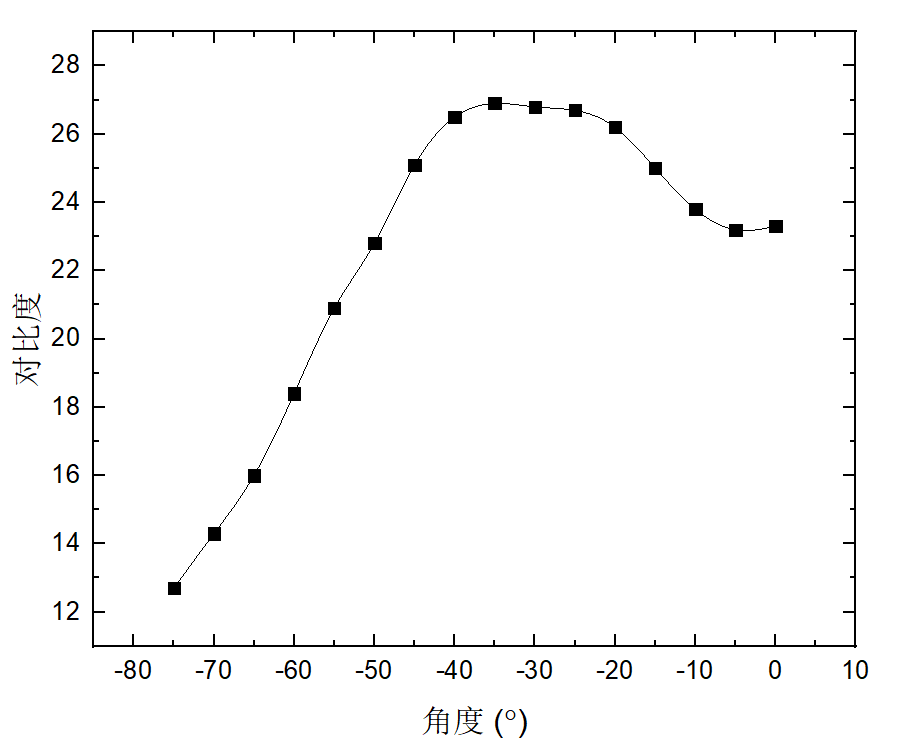
\includegraphics[scale=0.42]{水平负}}
		\subfigure[水平方向正角度]{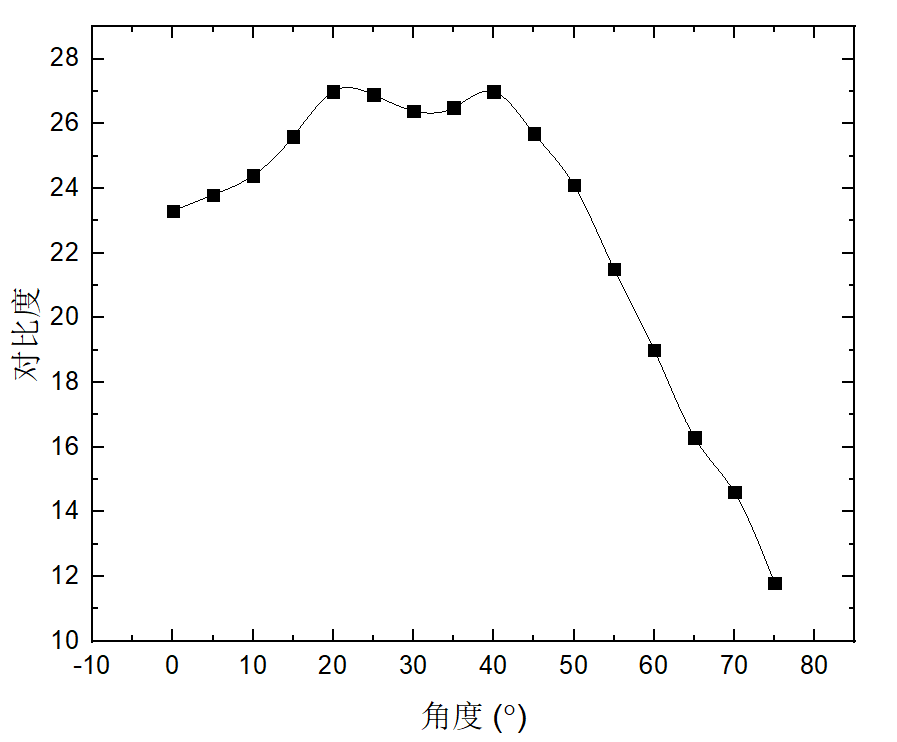
\includegraphics[scale=0.42]{水平正}}
		
		\subfigure[垂直方向负角度]{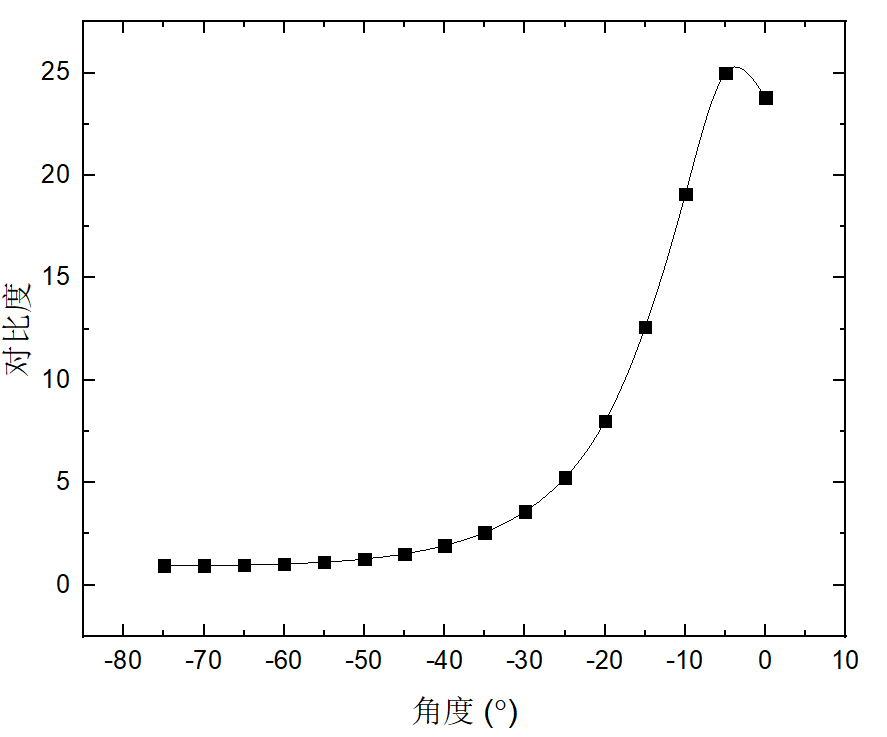
\includegraphics[scale=0.42]{垂直负}}
		\subfigure[垂直方向正角度]{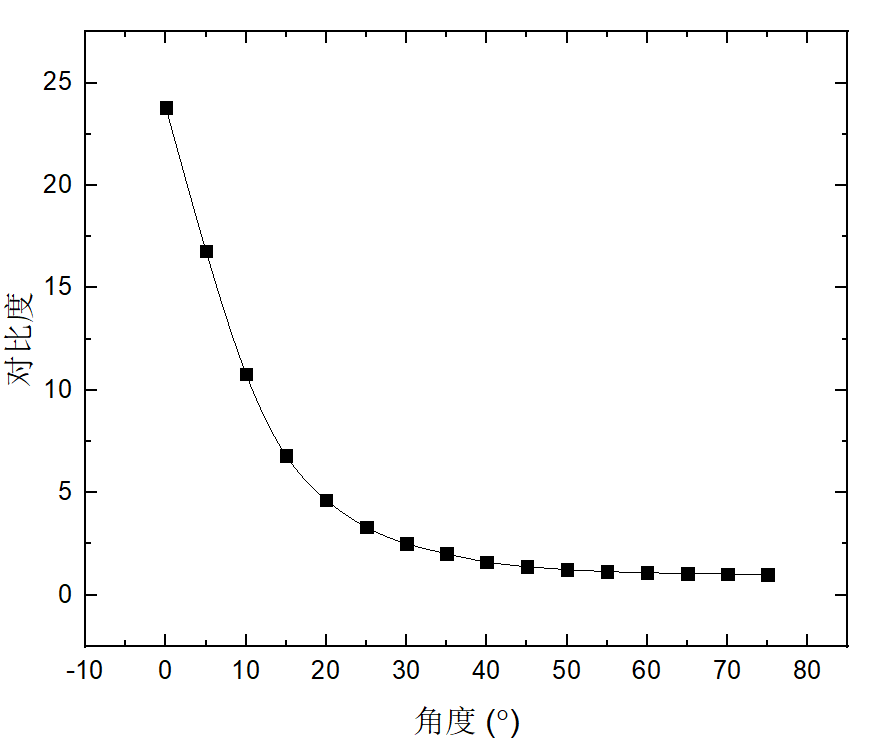
\includegraphics[scale=0.42]{垂直正}}
		\captionsetup{font={small},labelfont=bf}
		\caption{\heiti\zihao{-5}实验环境模拟图}
		
	\end{figure}
	
	\section{思考题和实验总结}
	\subsection{思考题}
	1.不加电压时,将液晶正对光源,校准为透光率$ 100\% $后,加上足够大的电压,若透光率下降,则为常白型。若不加电压时无光透过,提高电压,在液晶后观察发现光强变强,则为常黑型。
	
	
	2.CRT需要持续更新闪光点,发光不稳定,而液晶显示器只需要改变液晶排列结构,显示更稳定,同时能耗也更低;CRT需要离子束打在荧光屏上,产生电磁辐射,而液晶无辐射源;CRT需要离子束的发射、接收屏等装置,体型笨重,液晶显示器结构更简单,轻巧。
	
	
	3.计算得到$ \frac{1}{\tau_r}=22.36s^{-1} $,$ \frac{1}{\tau_d}=44.50s^{-1} $,$ 22.36<25 $,如达到标准应需要上升、下降时间的帧数都高于25,故不能。响应时间需要上升、下降时间均低于40ms。
	
	
	4.实验室在亮的环境下,可能是由于当角度旋转时,有从其他方向入射的来自实验室的背景光,在这些角度下对背景光的透过率有所提升,导致接收到的光强反而大于$ 100\% $。尤其对于我所在的试验台,刚好侧对着黑板屏幕显示器,在测量水平方向正角度时在锐角处明显存在这样的情况,一定角度范围内透过率一直维持在$ 100\% $。
	\subsection{实验总结}
	通过本实验了解了液晶的工作原理,测量了液晶显示的有关性质,并且通过实验测量得到了液晶视角特性明显的非对称性。此类光学实验最好可以在较暗的实验环境中进行,以获得更加准确的测量数据结果。
\end{document}